\section{Multi-level Snapshot Deduplication}
\label{sect:dedupe}

\subsection{Snapshot System}
%system arch
Our architecture is built on the Aliyun platform which provides the largest public VM cloud in China. 
A typical VM cluster in our cloud environment
consists of from hundreds to thousands of physical machines, each of which can
host tens of xen-based\cite{Barham2003} VMs.

Aliyun has built a hadoop-like platform, which includes
several highly scalable cloud infrastructure services to support
 runing large scale VM cloud service:
\begin{itemize}
\item \textbf{DFS}: a distributed file system that is optimized for many large and sequential reads or appends.
\item \textbf{KV}: a distributed key-value store for managing structured data.
\item \textbf{MP}: a distributed data processing framework which is similar to Map-Reduce\cite{Dean2004}.
\item \textbf{MemCache}: a distributed memory object caching system.
\end{itemize}
%GFS-like\cite{googlefs03} 
%BigTable-like\cite{Chang2008a} 
Our snapshot system and the virtual machine management service rely on these basic cloud services
to be functional:
DFS holds the responsibility of managing physical disk storage
in the cloud, all data needed for VM services, such as virtual disk images used by runtime VMs,
and snapshot data for backup purposes, reside in this distributed file system. 
In addition, our snapshot system 
places the index of CDS in MemCache for deduplication, 
stores small amount of snapshot metadata in KV, and uses FX to facilitate the offline
data processing. All the above services can easily find their open-source counterparts,
which shows the generality of our architecture and deduplication scheme.

User control VMs through the virtual machine management service.
During VM creation, a user chooses a pre-configured VM image or
a snapshot that contains an OS,
then the VM management service 
copies the corresponding VM image to her VM as the OS disk.
Data disks can be created and mounted onto the VM in the same way,
either empty or from an existing snapshot. 
All these virtual disks are represented as virtual disk image files in our
underline runtime VM storage system.  
To avoid network latency and congestion, 
our distributed file system place the primary replica of VM's 
image files at physical machine of VM instance.
When user deletes her VM, all the runtime virtual disk images and
their snapshot data are removed from DFS.

%ss operations
In each VM, 
the runtime I/O between virtual machine and its virtual
disks is tunneled by the virtual device driver (called TapDisk\cite{Warfield2005} at Xen).
This is also where our snapshot system is built in. Three major snapshot operations are supported:
\begin{itemize}
\item \textit{Write snapshot}: save the current state of virtual disk as a snapshot.
This is also where data deduplication would take place.
During snapshot backup, concurrent disk write is logged 
to ensure a consistent snapshot version is captured. 
\item \textit{Read snapshot}: restore the state of virtual disk from a snapshot.
\item \textit{Delete snapshot}: delete a snapshot and reclaim the disk space for unused data.
\end{itemize}

\begin{figure}[htbp]
  \centering
  %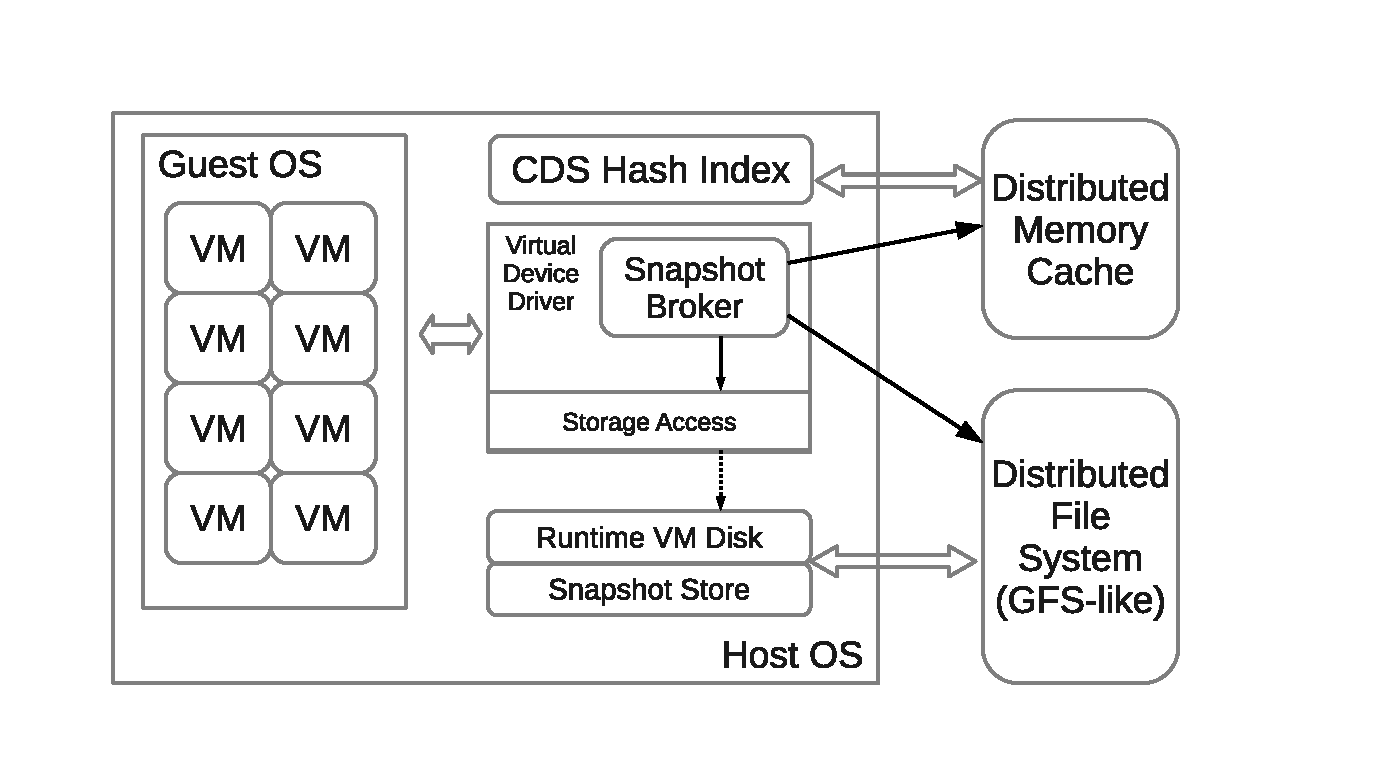
\epsfig{file=images/arch.eps, height=2in, width=2.66in}
  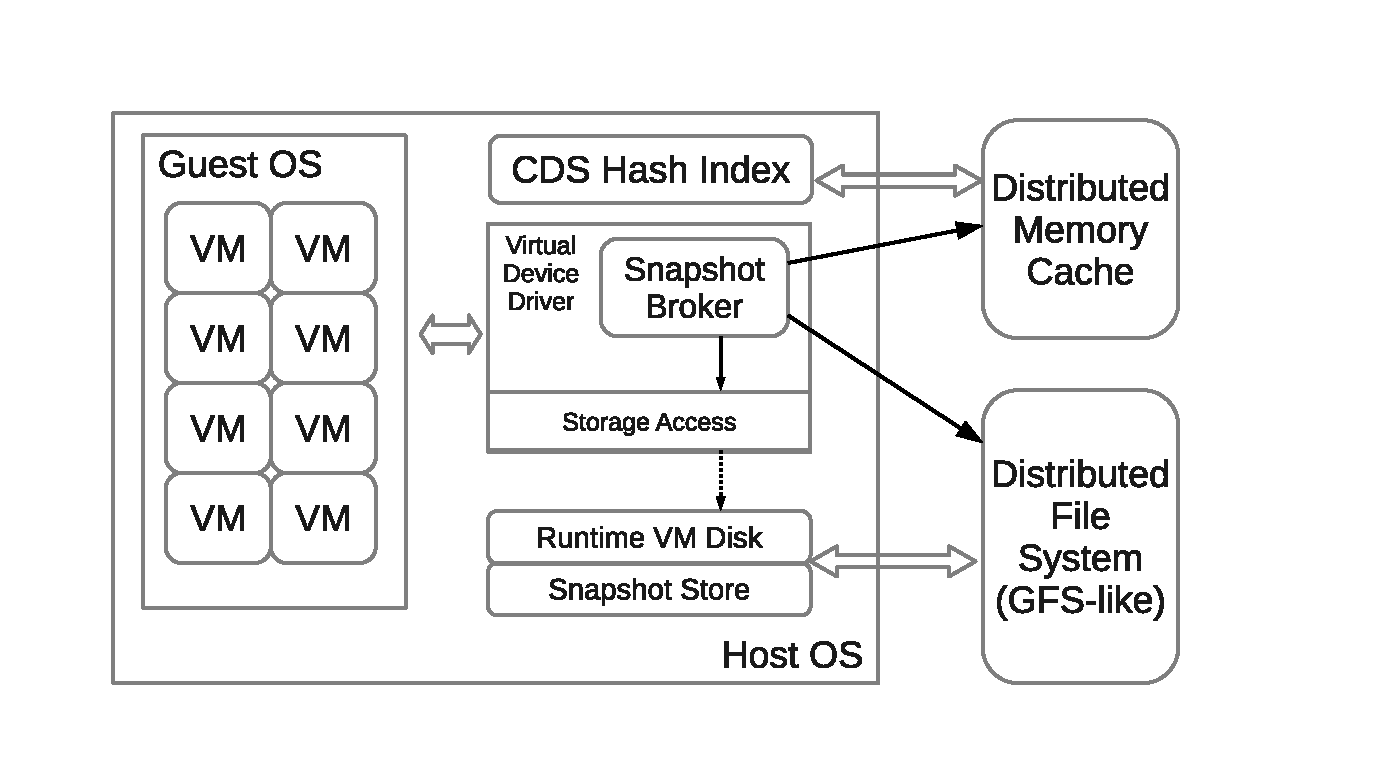
\epsfig{file=images/arch.eps, width=3.9in}
  \caption{Snapshot backup architecture of each node.}
  \label{fig:arch}
\end{figure}

Figure~\ref{fig:arch} shows the architecture view of our snapshot service
at each node. The snapshot broker provides the functional interface for  snapshot backup, access, and deletion.
The inner-VM  deduplication is conducted by the broker to access meta data in the snapshot data store
and we discuss this in details in Section~\ref{sect:innerVM}.
The cross-VM deduplication is conducted by the broker to access 
a common data set (CDS) (will discuss in Section~\ref{sect:crossVM},
whose block hash index is stored in a distributed memory cache. 

%snapshot representation
\subsection{Snapshot Representation}
The virtual device driver uses a bitmap to track the changes 
that have been made to virtual disk.
Every bit in the bitmap represents a fix-sized (2MB) region called \textit{segment}, indicates whether the segment
is modified since last backup. Hence we could treat segment as the basic unit in snapshot backup similar to
file in normal backup: a snapshot could share a segment with previous snapshot it is not changed. 
Moreover, we break 
segments into var-sized chunks (average 4KB) using content-based chunking algorithm,
which brings the opportunity of fine-grained deduplication by
allowing data sharing between segments.

\begin{figure}[htbp]
  \centering
  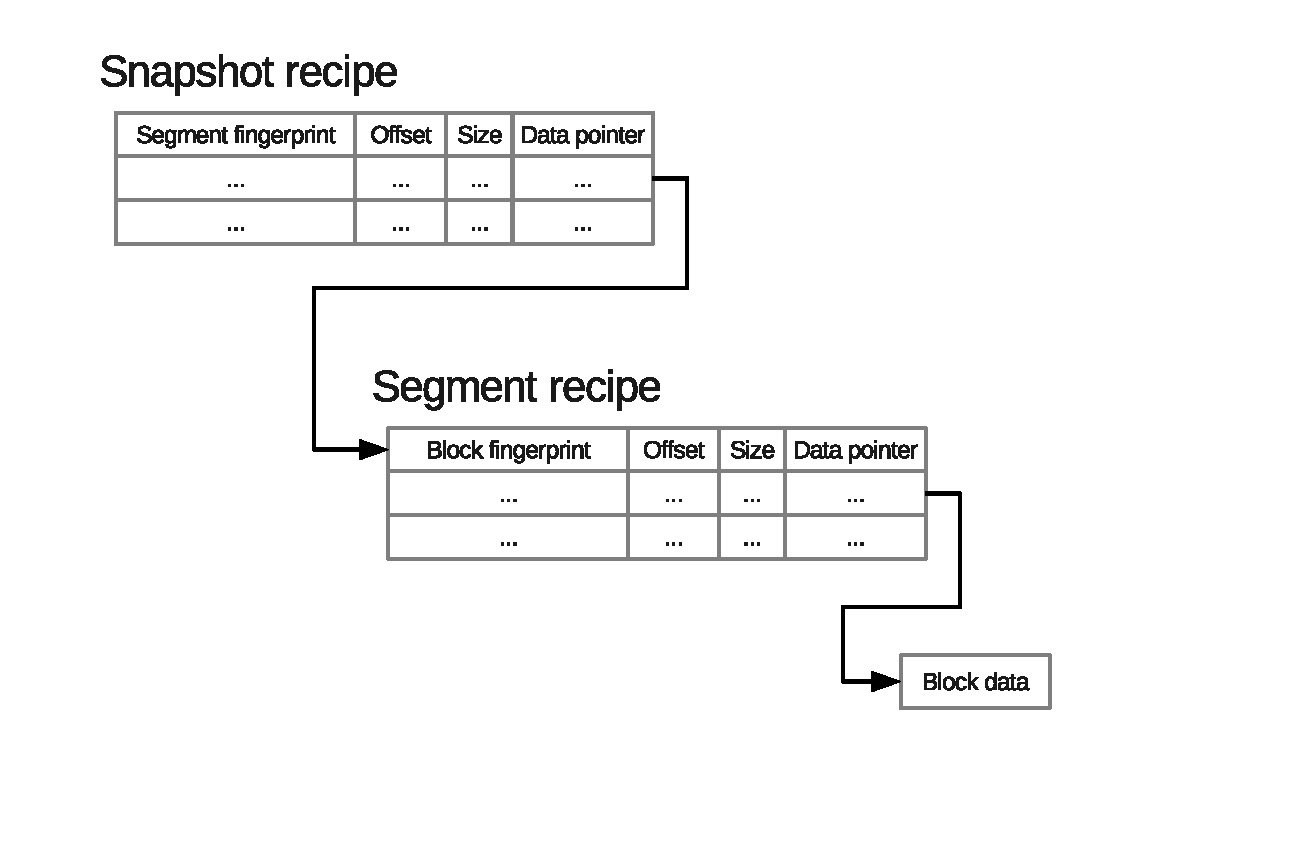
\epsfig{file=images/snapshot_representation.eps, width=3.7in}
  \caption{An example of snapshot representation.}
  \label{fig:snapshot}
\end{figure}
As a result, the representation of each snapshot is designed as a two-level index data structure 
in the form of a hierarchical directed acyclic graph as shown in Figure \ref{fig:snapshot}.
A snapshot recipe contains a list of segments, each of which is represented as a segment recipe
that holds the meatdata of its chunks. We choose this two-level structure because in practice we
observe that during each backup period only a small amount of VM data are added or modified. 
As the result, even the metadata of two snapshots can be highly similar, 
thus aggregating a large number of chunks as one segment can significantly reduce the space cost of snapshot metadata.
Furthermore, instead of using variables-sized segments, we use a dirty bit to capture the change status of fix-sized
segments which greatly ease the segment-level deduplication.

In both two kind of recipes, 
they do not include the actual data but only have
 references point to the data which are either stored in append store or CDS.
In our implementation the data reference is a 8 bytes field which is either an 
ASID (discuss in \ref{sect:append} or an offset of 
An additional flag indicates

\subsection{Multi-level Deduplication}
The multi-level deduplication scheme is designed base on the observations on the VM snapshot data from production cloud.
We found snapshot data duplication can be easily classified into two categories: \textit{Inner-VM} and \textit{Cross-VM}. 
Inner-VM duplication exists between VM's snapshots, because the majority of data are unchanged during each backup period. 
On the other hand, Cross-VM duplication is mainly due to widely-used software and libraries such as Linux and MySQL. 
As the result, different VMs tend to backup large amount of highly similar data.
Our multi-level pipeline process can minimize the cost of deduplication while maximize the its efficiency at each level,
and it is highly parallelizable since each segment is processed independently.

\subsubsection{Inner-VM Deduplication}
\label{sect:InnerVM}
The first-level deduplication is logically localized within each VM.
Such localization increases data independency between different VM backups,
simplifies snapshot management and statistics collection,
and facilitates parallel execution of snapshot operations.

The inner VM deduplication contains two levels of duplicate detection efforts:
\begin{itemize}
\item \textit{Level 1 Segment modification detection}.
If a segment is not changed, then its segment recipe can be simply reused by copying the data
reference from previous snapshot recipe. 
\item \textit{Level 2  Chunk fingerprint comparison.}
If a segment is modified, we perform fine-grained deduplication 
by comparing the fingerprints of its chunks to the same segment's recipe in the previous snapshot,
thus eliminate partial data duplication within the segment.
\end{itemize}

In general, operations at level 1 have almost no cost and most of unmodified data are filtered here. 
To process a dirty segment at level 2, 
there requires no more than one DFS access to load the segment recipe from previous snapshot,
and a tiny amount of memory to hold it in main memory.
\textit{may need details here}

\subsubsection{Cross-VM Deduplication}
\label{sect:CrossVM}

\subsection{Common Data Set}
%arch
%analysis